\section{Interfejs analogowy}

Drugą z~zaimplementowanych sekcji projektu był interfejs analogwy, który umożliwić miał odczyt wartości napięć na~potencjometrach z~wykorzystaniem zewnętrznego multipleksera analogowego. Zdecydowano się wykorzystać w~tym celu generator IPC (ang. \textit{Intelectual Property Core}) \textit{XADC Wizard} (wersja 3.3). Prace rozpoczęto od zapoznania się zarówno z~dokumentacją modułu ADC dostępnego w~układach FPGA serii sióddmej (\cite{xilinx_adc_series_seven}) jak i~samego generatora (\cite{xilinx_xadc_wizard}). Z~ich pomocą udało się rozszyfrować znaczenie poszczególnych parametrów rdzenia. Zdecydowano się na wykorzystanie interfejsu DRP (ang. \textit{Dynamic Reconfigurable Port}) ze względu na jego relatywną prostotę. XADC został skonfigurowany w~trybie sekwencyjnym (ang. \textit{channel sequencer}) z~manualnym wyzwalanym (ang. \textit{event mode}). Prędkość sygnału zegarowego przyjęto na poziomie 100MHz (zgodnie z~założeniami projektu) natomiast częstotliwość konwersji na poziomie 50KSPS (ang. \textit{KiloSamples Per Second}). Dodatkowo skorzystano z~udostępnianej przez XADC możliwości automatycznego wysterowania linii \textit{select} zewnętrznego multipleksera analogowego. Jako kanał roboczy wybrano \textit{vaux0}, który skonfigurowano w~trybie unipolarnym. Zrezygnowano z~uśredniania wartości próbek w~kanałach oraz dezaktywowano wszystkie alarmy. Ostatnim krokiem było ustawienie odpowiednich wartości w~sekcji \textit{Analog Sim Options} zakładki \textit{Basic}. Wpisano w~niej ścieżkę do zewnętrznęgo pliku zawierającego przebiegi symulowanych wartości analogowych. Jak się później okazało sfinalizowanie tej konfiguracji celem uzyskania możliwości uruchomienia rzeczonej symulacji wymagało spędzenia dodatkowych kilku godzin na przeglądaniu forum \verb|forum.xilinx.com| celem odszukania informacji brakujących w~dokumentacji.

\vspace{0.5cm}
\begin{figure}[ht]
    \centering
    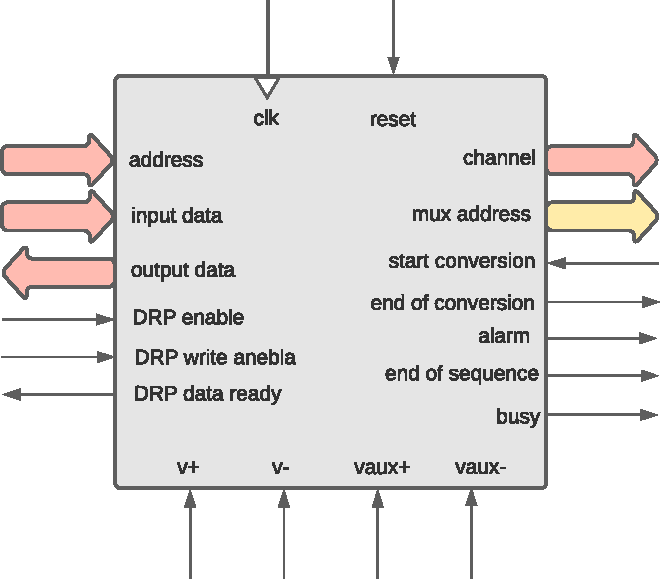
\includegraphics[scale=0.8]{img/diagrams/xadc.pdf}
    \captionsetup{format=plain,justification=centering}
    \caption{Struktura portów wygenerowanego modułu XADC}
    \label{xadc-structure}
\end{figure}
\vspace{0.5cm}

Strukturę wyprowadzeń wygenerowanego bloku funkcjonalnego przedstawiono na Rys. \ref{xadc-structure}. Po lewej stronie przedstawiono sygnały związane z~odczytem i~zapisem wewnętrznych rejestrów modułu. Na dolnej krawędzi znalazły się bipolarne wejścia analogowe. Znaczenie sygnałów zaprezentowanych naprawej krawędzi są następujące:

\begin{itemize}
    \item \textit{channel} - port wyjściowy reprezentujący adres rejestru zawierającego dane z~ostatniego kanału spróbkowanego przez XADC; ustawiany jest na końcu konwersji (niewykorzystany w~projekcie)
    \item \textit{mux address} - linie wysterowujące wejścia \textit{select} zewnętrznego multipleksera analogowwego
    \item \textit{start conversion} - linia aktywujące nową konwersję
    \item \textit{end of conversion} - linia ustawiana w~stan wysoki na jeden takt zegara po zakońćzeniu konwersji
    \item \textit{alarm} i~\textit{end of sequence} - linie alaramu oraz sygnalizacji końca sekwencji aktywne w~stanie wysokim (nieużywane w~projekcie)
    \item \textit{busy} - linia ustawiana w~stan wysoki na czas trwania konwersji
\end{itemize}

Wokół tak rpzedstawiającej się struktury stworzony został prosty moduł interfejsujący, który automatyzuje cykliczne wyzwalania konwersji oraz odczyt danych z~wewnętrznych rejestrów XADC. Jego struktura ostała przedstawiona na Rys. \ref{analog-scanner-structure}. Port \verb|data| reprezentowany jest przez tablicę N~wektorów 12-bitowych ($N <= 16$) odzwierciedlających wartości napięcia na kolejnych kanałach multipleksera. W~projekcie wykorzystano dziewięć kanałów (dziewięć potencjometrów), których znaczenie przedstawiono w~dalszej części dokumentu. Na zewnątrz modułu wystawione zostały poza tym wejścia analogowe kanału \textit{vaux0} (oznaczone omyłkowo jako wyjścia) oraz linie \textit{select} dla zewnętrznego multipleksera. Dedykowane wejścia analogowe (\textit{vp/vn}) zostały podłączone na stałe do masy. Parametry (ang.\textit{generic}) modułu pozwalają skonfigurować ilość wykorzystywanych kanałów\footnote{Musi być zgodna z~konfiguracją podaną na etapie generowania XADC} oraz częstotliwość próbkowania kanałów.
 
\vspace{0.5cm}
\begin{figure}[ht]
    \centering
    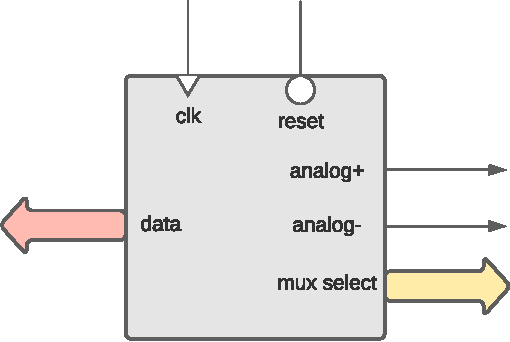
\includegraphics[scale=1.0]{img/diagrams/analog_scanner.pdf}
    \captionsetup{format=plain,justification=centering}
    \caption{Struktura portów bloku skanera kanałów analogowych}
    \label{analog-scanner-structure}
\end{figure}
\vspace{0.5cm}

Zasada działania modułu zasadza się na dwóch synchronicznych procesach. Pierwszy z~nich wyposażony jest w~wewnętrzny licznik, który odmierza takty zegara systemowego między kolejnymi konwersjami. Gdy jego wartość spadnie do zera linia \verb|start conversion| bloku XADC zostaje ustawiona w~stan wysoki na jeden cykl zegara. Równolegle wartość wyjścia \verb|mux address| - powiększona o~wartość $0$x$10$ (adres danych pierwszego kanału pomocniczego \textit{vaux0}) - zostaje przepisana na wejście adresowe interfejsu DRP. Drugi proces implementuje dwustanowy automat skończony. W~pierwszym ze stanów proces oczekuje na pojawienie się stanu wysokiego na linii \verb|end of conversion|. Gdy sytuacja ta zajdzie, linia \verb|DRP enable| również ustawiana jest w~stan wysoki, co rozpoczyna odczyt danych spod adresu znajdującego się na liniach adresowych (ustawianych przez pierwszy proces). Akcja finalizowana jest przejściem do drugiego stanu, w~którym proces pozostaje do wystwaienia przez XADC logicznej jedynki na linii \verb|DRP ready| oznaczającej pojawienie się odczytanych danych na procie \verb|output data|. Dane te kopowiane są do odpowiedniego wektora w~tablicy \verb|data| i~proces przechodzi ponownie do stanu pierwszego.

\vspace{0.5cm}
\begin{figure}[ht]
    \centering
    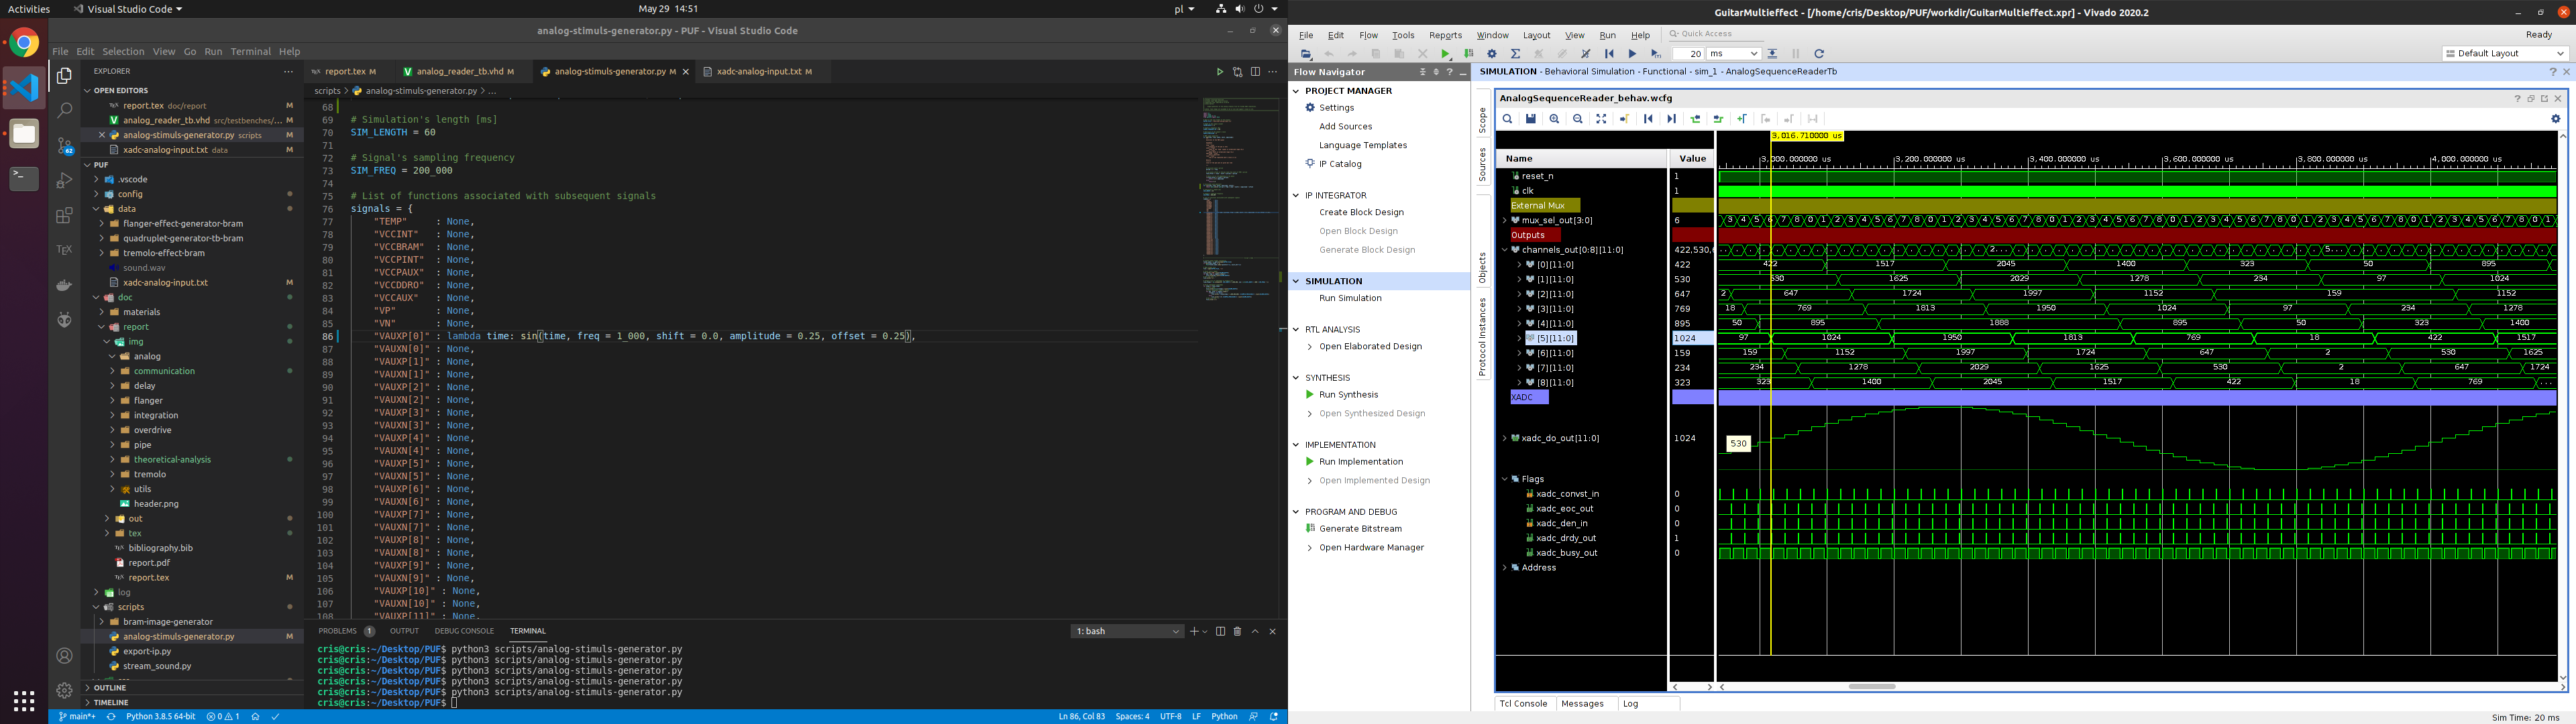
\includegraphics[width=\textwidth]{img/sim/analog_scanner_sim.png}
    \captionsetup{format=plain,justification=centering}
    \caption{Fragment symulacji bloku skanera analogowego}
    \label{sim-analog-scanner}
\end{figure}
\vspace{0.5cm}

W~celu weryfikacji zaimplementowanego rozwiązania ponownie przygotowano stosowną symulację. Tym razem weryfikacja nie miała charakteru formalnego, tzn. efekty działania testowanego modułu nie były programowo porównywane z~wartościami oczekiwanymi. Ze względu na złożoność implementacji takiego rozwiązania ograniczono się jedynie do weryfikacji jakościowej poprzez manualną analizę zasymulowanych przebiegów. Aby jednak symulacja była możliwa należało najpierw stworzyć odpowiedni plik zawierający przebiegi wartości napięcia na kolejnych kanałach ADC. Generację takowego pliku zautomatyzowano za pomocą prostego skryptu języka Python, który pozwala zdefiniować długość trwania generowanych sygnałów, ich przebieg oraz częstotliwość ``próbkowania''. Z~jego pomocą wygenerowano sinusoidalny przebieg napięcia na kanale \textit{vauxp0} ustawiając jednocześnie pozostałe kanały na wartość~$0$. Fragment symulacji obrazuje Rys. \ref{sim-analog-scanner}. Przyjęto w~niej częstotliwość konwersji na maksymalnym poziomie 50KSPS. Jak widać wektory tabeli \textit{channels\_out} (podłączej do portu wyjściowego \verb|data| skanera) są aktualizowane w~zakładany sposób. Dla lepszego zobrazowania sposobu działania układy rysunek ukazuje także bezpośrednie przebiegi niektórych portów modułu XADC. 
